% This file was created by matlab2tikz.
%
%The latest updates can be retrieved from
%  http://www.mathworks.com/matlabcentral/fileexchange/22022-matlab2tikz-matlab2tikz
%where you can also make suggestions and rate matlab2tikz.
%
\definecolor{mycolor1}{rgb}{0.00000,0.44700,0.74100}%
\definecolor{mycolor2}{rgb}{0.92900,0.69400,0.12500}%
\definecolor{mycolor3}{rgb}{0.46600,0.67400,0.18800}%
\definecolor{mycolor4}{rgb}{0.63500,0.07800,0.18400}%
\definecolor{mycolor5}{rgb}{0.85000,0.32500,0.09800}%
%
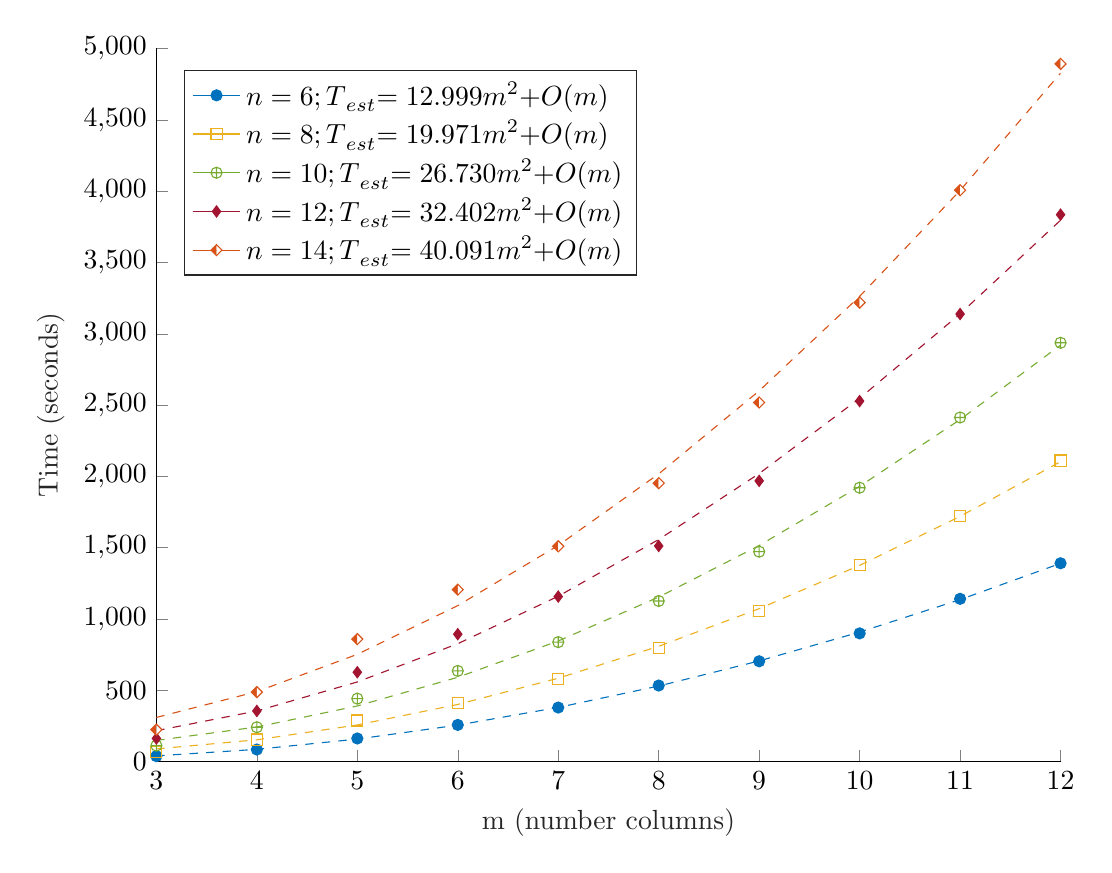
\begin{tikzpicture}

\begin{axis}[%
width=4.521in,
height=3.566in,
at={(0.758in,0.481in)},
scale only axis,
xmin=3,
xmax=12,
xlabel style={font=\color{white!15!black}},
xlabel={m (number columns)},
ymin=0,
ymax=5000,
ylabel style={font=\color{white!15!black}},
ylabel={Time (seconds)},
axis background/.style={fill=white},
title style={font=\bfseries},
% title={$\text{Average ticks until solution as a function of m. On n }\times\text{ m grid. (k = 5)}$},
axis x line*=bottom,
axis y line*=left,
legend style={at={(0.03,0.97)}, anchor=north west, legend cell align=left, align=left, draw=white!15!black}
]
\addplot [color=mycolor1, draw=none, mark=*, mark options={solid, mycolor1}]
  table[row sep=crcr]{%
3	38.922\\
4	85.334\\
5	162.84\\
6	257.966\\
7	379.72\\
8	533.968\\
9	704.074\\
10	899.646\\
11	1141.9\\
12	1391.172\\
};
\addlegendentry{$\text{n =  6; T}_{\text{est}}\text{ = 12.999m}^\text{2}\text{ + }O(\text{m})$}

\addplot [color=mycolor1, dashed, forget plot]
  table[row sep=crcr]{%
3	40.73536363636\\
4	86.7016909090896\\
5	158.665548484849\\
6	256.626936363638\\
7	380.585854545457\\
8	530.542303030305\\
9	706.496281818184\\
10	908.447790909092\\
11	1136.39683030303\\
12	1390.3434\\
};
\addplot [color=mycolor2, draw=none, mark=square, mark options={solid, mycolor2}]
  table[row sep=crcr]{%
3	70.482\\
4	155.078\\
5	288.784\\
6	413.962\\
7	579.478\\
8	796.068\\
9	1054.262\\
10	1377.316\\
11	1722.83\\
12	2111.108\\
};
\addlegendentry{$\text{n =  8; T}_{\text{est}}\text{ = 19.971m}^\text{2}\text{ + }O(\text{m})$}

\addplot [color=mycolor2, dashed, forget plot]
  table[row sep=crcr]{%
3	89.680945454544\\
4	153.669115151514\\
5	257.599709090909\\
6	401.472727272727\\
7	585.28816969697\\
8	809.046036363637\\
9	1072.74632727273\\
10	1376.38904242424\\
11	1719.97418181818\\
12	2103.50174545455\\
};
\addplot [color=mycolor3, draw=none, mark=oplus, mark options={solid, mycolor3}]
  table[row sep=crcr]{%
3	112.686\\
4	241.676\\
5	442.154\\
6	636.586\\
7	838.246\\
8	1126.738\\
9	1472.368\\
10	1920.808\\
11	2413.222\\
12	2936.758\\
};
\addlegendentry{$\text{n = 10; T}_{\text{est}}\text{ = 26.730m}^\text{2}\text{ + }O(\text{m})$}

\addplot [color=mycolor3, dashed, forget plot]
  table[row sep=crcr]{%
3	149.249345454545\\
4	243.328606060606\\
5	390.867715151515\\
6	591.866672727273\\
7	846.325478787879\\
8	1154.24413333333\\
9	1515.62263636364\\
10	1930.46098787879\\
11	2398.75918787879\\
12	2920.51723636364\\
};
\addplot [color=mycolor4, draw=none, mark=diamond*, mark options={solid, mycolor4}]
  table[row sep=crcr]{%
3	162.898\\
4	355.852\\
5	627.17\\
6	893.99\\
7	1157.482\\
8	1512.326\\
9	1968.836\\
10	2528.112\\
11	3138.58\\
12	3835.148\\
};
\addlegendentry{$\text{n = 12; T}_{\text{est}}\text{ = 32.402m}^\text{2}\text{ + }O(\text{m})$}

\addplot [color=mycolor4, dashed, forget plot]
  table[row sep=crcr]{%
3	217.40690909092\\
4	355.847503030307\\
5	559.092248484848\\
6	827.141145454541\\
7	1159.99419393939\\
8	1557.65139393939\\
9	2020.11274545454\\
10	2547.37824848485\\
11	3139.44790303031\\
12	3796.32170909092\\
};
\addplot [color=mycolor5, draw=none, mark=halfsquare left*, mark options={solid, mycolor5}]
  table[row sep=crcr]{%
3	224.602\\
4	487.724\\
5	859.618\\
6	1206.27\\
7	1510.346\\
8	1952.838\\
9	2518.19\\
10	3218.688\\
11	4006.49\\
12	4892.054\\
};
\addlegendentry{$\text{n = 14; T}_{\text{est}}\text{ = 40.091m}^\text{2}\text{ + }O(\text{m})$}

\addplot [color=mycolor5, dashed, forget plot]
  table[row sep=crcr]{%
3	310.260309090919\\
4	491.425896969701\\
5	752.772863636363\\
6	1094.30120909091\\
7	1516.01093333333\\
8	2017.90203636363\\
9	2599.97451818181\\
10	3262.22837878788\\
11	4004.66361818182\\
12	4827.28023636364\\
};
\end{axis}
\end{tikzpicture}%
